{\begin{a3pages}
% ---------------------------------------------------------------------------- %
\clearpage
\section{Sensorplatine}
\label{sec:hw:sensorplatine}
% ---------------------------------------------------------------------------- %
    \setlength{\parindentbak}{\parindent}

    \noindent\adjustbox{valign=t}{\begin{minipage}{135mm}
        Das Sensorboard besteht aus einer CPU welche alle Komponenten koordiniert, einem Modulator und einem Demodulator zur Kommunikation, einem Buck-Konverter der die Netzspannung f\"ur das Board transformiert.

        Als CPU dient ein Atmel SAM D09. Dieser wurde gew\"ahlt da er die g\"unstigste CPU in seiner Klasse ist und alle notwendigen Features mitbringt. (3)
        Der Mikrochip hat einen 12 Bit ADC, ein CRC Modul, hat eine 32 Bit ARM Architektur und braucht extrem wenig Leistung.

        Zum Speisen des Boardes wird ein LMR16006 verwendet. Dieser kann die volle Spanne von 12 Volt bis 60 Volt ohne Probleme auf 3.3 Volt regeln, welche das Board versorgen. (1)

        Als Modulator dient ein Voltage Controlled Oscillator (VCO) auf dem 74HC4640 Chip von Texas Instruments.
        Dieser kann mit der richtigen Beschaltung Frequenzen zwischen wenigen Kilohertz bis mehrere Megahertz erzeugen.(2)

        Zum Demodulieren wird ein einfaches Tiefpassfilter mit einer Diode und einem Verst\"arker benutzt.(6)

        Und nat\"urlich hat es einen Spannungsteiler zum Messen der Versorgungsspannung. (4)

        Im Folgenden sind die einzelnen Komponenten dokumentiert und ihre Wahl begr\"undet.

        \adjustbox{valign=t}{\begin{minipage}{0.475\textwidth}
            \centering
            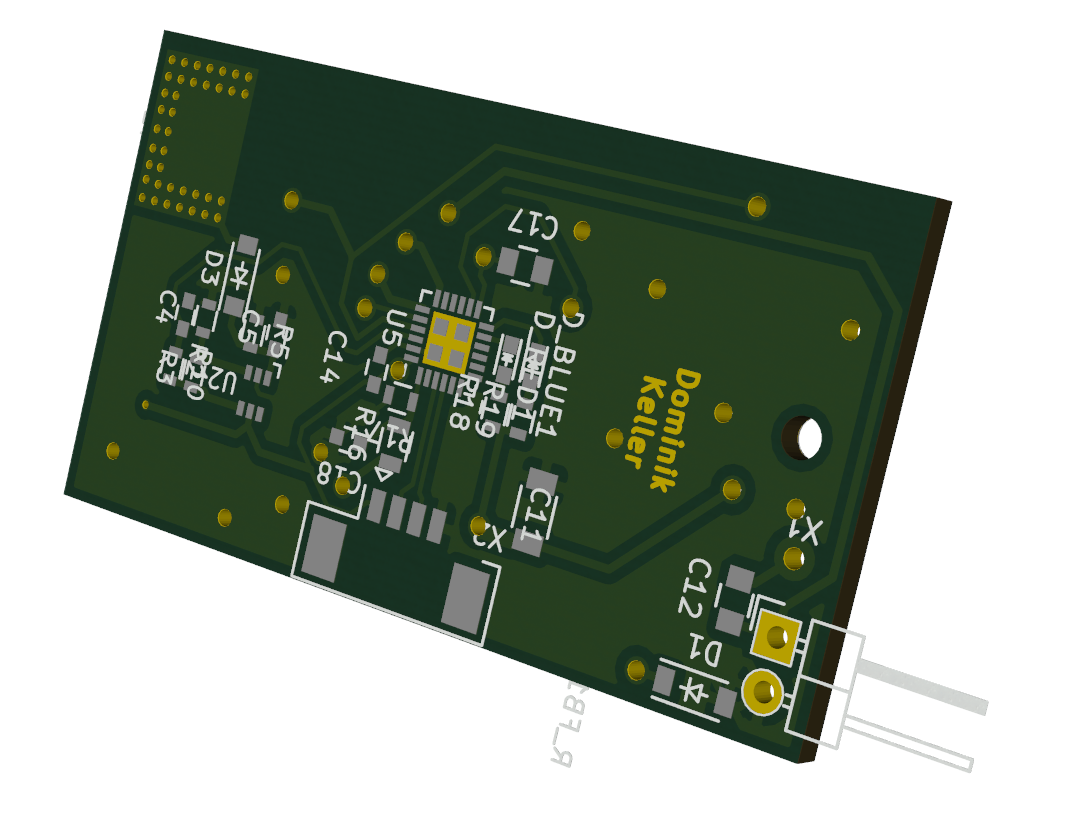
\includegraphics[width=0.9\textwidth]{images/sensor-pcb/sensor-3d-front.png}
            \figcaption[Sensor: Vorderseite PCB]{PCB, Vorderseite}
            \label{fig:sensor:pcb:front}
        \end{minipage}}
        \adjustbox{valign=t}{\begin{minipage}{0.475\textwidth}
            \centering
            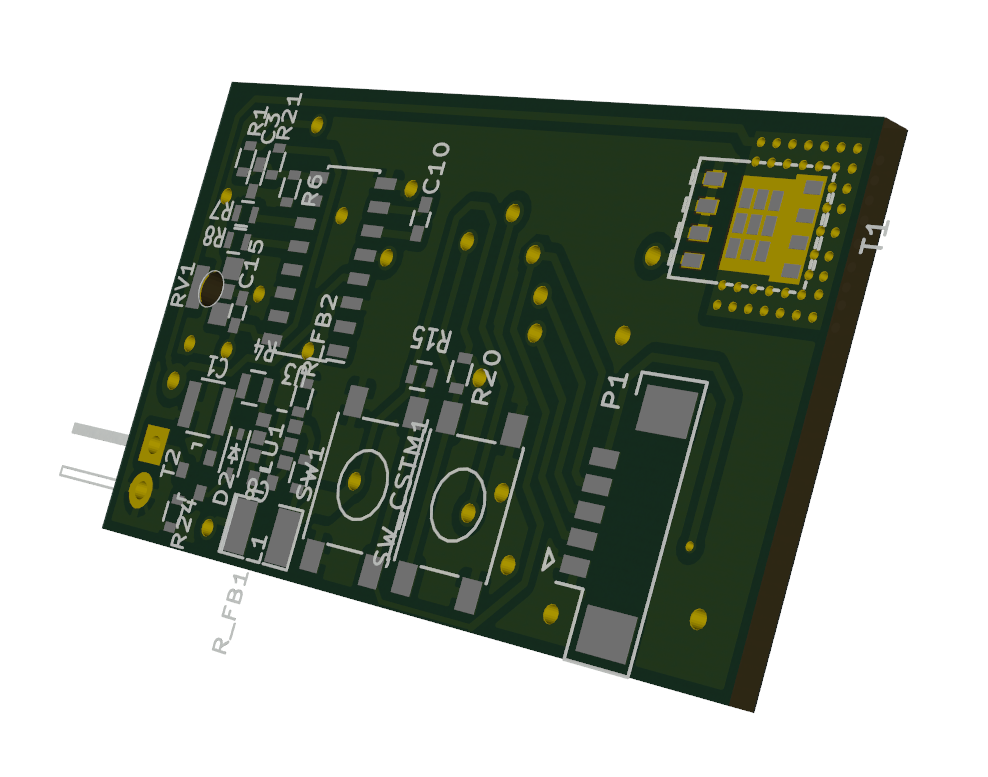
\includegraphics[width=0.9\textwidth]{images/sensor-pcb/sensor-3d-back.png}
            \figcaption[Sensor: R\"uckseite PCB]{PCB, R\"uckseite}
            \label{fig:sensor:pcb:back}
        \end{minipage}}
    \end{minipage}}
    \hspace*{15mm}
    \adjustbox{valign=t}{\begin{minipage}{195mm}
        \centering
        \includegraphics[width=\textwidth]{images/sensor-sch/sensor--sch--highlights.eps}%
        \figcaption[Schema Sensor, \"Ubersicht]{%
            Schema   des   \Sensor   s. Eine  Grossversion   ist   in   Anhang
            \label{app:chap:schemas}  zu  finden,   die  einzelnen  Baugruppen
            sind  in  den  folgenden  Abschnitten  beschrieben  und  gr\"osser
            abgebildet.%
        }
        \label{fig:sensor:schema:highlights}
    \end{minipage}}
\end{a3pages}}


% ---------------------------------------------------------------------------- %
\subsection{Speisung}
\label{subsec:hw:sensor:supply}
% ---------------------------------------------------------------------------- %

Die Speisung der Schaltung übernimmt ein LMR16006. Er ist bis 63 Volt input rated, das heisst es ist noch ein wenig Spiel zu den 60 Volt welche am Einganz anliegen können. Er kommt auch mit 4 Volt am Eingang noch klar. Da die Versorgungsspannung zwischen 12 Volt und 60 Volt schwankt durch den Tag, ist der LMR16006 soweit bestens geeignet.
Er hat einen sehr konstanten Wirkungsgrad von 70 bis 80 Prozent, je nach Speisespannung.
Der LMR16006 kann maximal 600 Miliampere liefern was ausreicht wenn man einen genug grossen Puffercap für Powerspikes einberechnet.
Zudem hat dieser Spannungsregler einen typischen Quiescent Current von nur 28 Mikroampere. Damit ist er auch extrem Stromsparend.
Die Beschaltung wurde nach Empehlung des Datenblatts gewählt, welche garantiert dass Powerspikes gut gefangen werden. $R_{FB1}$ und $R_{FB2}$ wurden explizit im Verhältnis $1:3.3$ gewählt, da 3.3 Volt die Spannung ist, die wir am Ausgang anstreben.

Der Active Low Shutdown Pin wird dauernd auf High gezogen, damit der Regler immer an ist sobald am Eingang Spannung anliegt.

Damit die Montage einfacher ist, ist ein Verpolungsschutz eingebaut. Dieser besteht aus einem P-Fet, einer Zenerdiode und einem Gate-Vorwiderstand.

\begin{figure}[h!t]
    \centering
    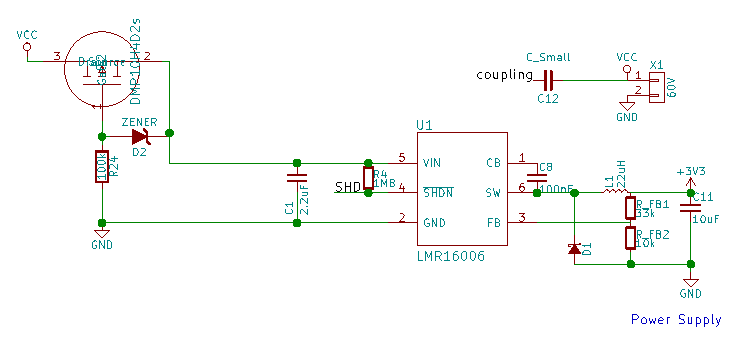
\includegraphics[width=1\textwidth]{images/sensor-sch/sensor--sch--supply.eps}
    \caption[Sensor: Schema Speisung]{Speisung Sensor}
\end{figure}

% ---------------------------------------------------------------------------- %
\subsection{Transmitter}
\label{subsec:hw:sensor:transmitter}
% ---------------------------------------------------------------------------- %

Der Transmitter besteht aus einem einfachen VCO der das Signal auf die Spannungsversorgung aufmoduliert.


\begin{figure}[h!t]
    \centering
    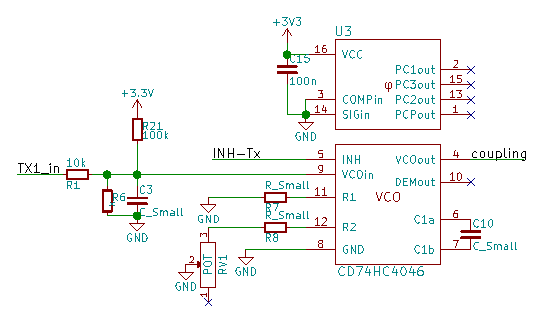
\includegraphics[width=1\textwidth]{images/sensor-sch/sensor--sch--transmitter.eps}
    \caption[Sensor: Schema Transmitter]{Transmitter Sensor}
\end{figure}

\todo{R1, R21, RV1, R7, R8, C10, C15}


% ---------------------------------------------------------------------------- %
\subsection{Microcontroller}
\label{subsec:hw:sensor:mcu}
% ---------------------------------------------------------------------------- %

\begin{figure}[h!t]
    \centering
    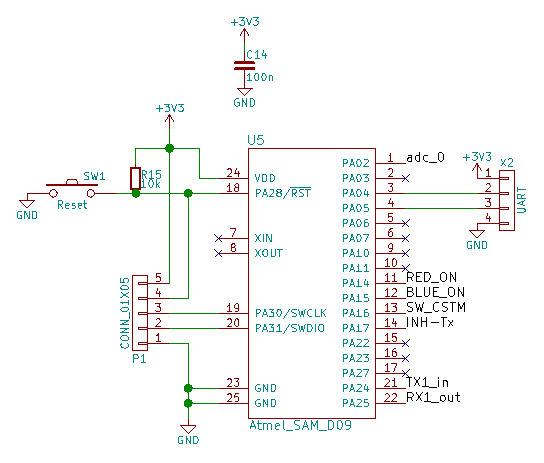
\includegraphics[width=0.5\textwidth]{images/sensor-sch/sensor--sch--mcu.eps}
    \caption[Sensor: Schema Microcontroller]{Microcontroller Sensor}
\end{figure}

\todo{R15, C14, Atmel Chip}

% ---------------------------------------------------------------------------- %
\subsection{Spannungsmessung}
\label{subsec:hw:sensor:voltageSense}
% ---------------------------------------------------------------------------- %

\begin{figure}[h!t]
    \centering
    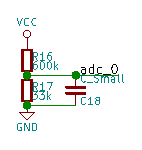
\includegraphics[width=0.5\textwidth]{images/sensor-sch/sensor--sch--sensor.eps}
    \caption[Sensor: Schema Spannungsmessung]{Spannungsmessung Sensor}
\end{figure}

\todo{R16, R17, C18}

% ---------------------------------------------------------------------------- %
\subsection{Interface}
\label{subsec:hw:sensor:interface}
% ---------------------------------------------------------------------------- %

\begin{figure}[h!t]
    \centering
    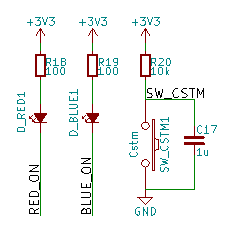
\includegraphics[width=0.5\textwidth]{images/sensor-sch/sensor--sch--interface.eps}
    \caption[Sensor: Schema Interface]{Interface Sensor}
\end{figure}

\todo{C17, R18, R19, R20}

% ---------------------------------------------------------------------------- %
\subsection{Empf\"anger}
\label{subsec:hw:sensor:receiver}
% ---------------------------------------------------------------------------- %

\begin{figure}[h!t]
    \centering
    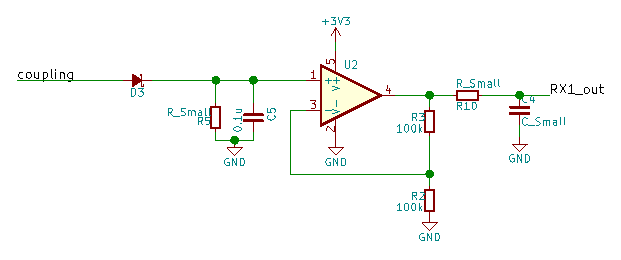
\includegraphics[width=0.5\textwidth]{images/sensor-sch/sensor--sch--receiver.eps}
    \caption[Sensor: Schema Empf\"anger]{Empf\"anger Sensor}
\end{figure}

\todo{R5, D3, C5, R3, R2, R10, C4, U2}
